\chapter{Analysis of Survival Times} \index{general}{survival times}

When analyzing survival times, different problems come up than the ones discussed so far. One question is how do we deal with subjects dropping out of a study. For example, assume that we test a new cancer drug. While some subjects die, others may believe that the new drug is not effective, and decide to drop out of the study before the study is finished.
A similar problem would be faced when we investigate how long a machine lasts before it breaks down.

\section{Survival Probabilities}

\subsection{Kaplan-Meier survival curve} \index{general}{Kaplan-Meier survival curve}

A clever way to deal with these problems is described in detail in \cite{altman99}. First, the time is subdivided into small periods. Then the likelihood is calculated that a subject survives a given period. The survival probability is given by

\begin{equation}
  p_k = p_{k-1} * \frac{r_k-f_k}{r_k}
\end{equation}

where $p_k$ is the probability to survive period $k$; $r_k$ is the number of subjects still at risk (i.e. still being followed up) immediately before the $k^{th}$ day, and $f_k$ is the number of observed failures on the day $k$. The curve describing the resulting survival probability is called \emph{life table}, \emph{survival curve}, or \emph{Kaplan-Meier curve} (see Figure \ref{fig:SurvivalCurve}).

\begin{figure}
  \centering
  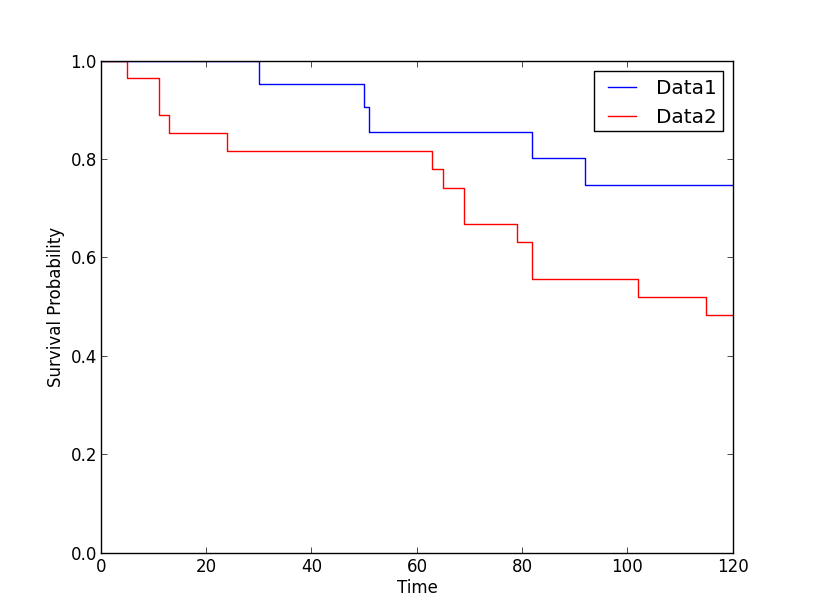
\includegraphics[width=0.5\textwidth]{../Images/Survival.png}\\
  \caption{Survival curve corresponding to a motion sickness experiment, described in more detail in \cite{altman99}, chapter 13}\label{fig:SurvivalCurve}
\end{figure}

Note that the survival curve changes only when a "failure" occurs, i.e. when a subject dies. \emph{Censored} entries, describing either when a subject drops out of the study or when the study finishes, are taken into consideration at the "failure" times, but otherwise do not affect the survival curve.

\section{Comparing Survival Curves in Two Groups} \index{general}{test!logrank}

The most common test for comparing independent groups of survival times is the \emph{logrank test}. This test is a non-parametric hypothesis test, testing the probability that both groups come from the same underlying population. Since to my knowledge this test is not yet implemented in a Python library, I have included an implementation based on the equations given by \cite{altman99} (see program \ref{py:survival}).

To explore the effect of different variables on survival, more advanced methods are required. The \emph{Cox regression model}\index{general}{Cox regression model} introduced by Cox in 1972 is used widely when it is desired to investigate several variables at the same time. For details, check \cite{altman99} or other statistic textbooks.

\PyImg "survival.py" (p \pageref{py:survival}): Survival analysis (Kaplan-Meier curves).
\index{python}{survival}
